\documentclass{article}
\usepackage{graphicx} % Required for inserting images
\usepackage{amsmath}
\usepackage{amsthm} 
\usepackage{amsfonts}
\usepackage{float}
\theoremstyle{definition}
\newtheorem*{sol}{Solution}
\usepackage{crimson}
\usepackage[a4paper,width=150mm,top=25mm,bottom=25mm]{geometry}
\usepackage{fancyhdr}

\pagestyle{fancy}
\fancyhf{}
\fancyhead[R]{Awez}
\fancyhead[L]{Exercise 1}
\fancyfoot[C]{\thepage}


\title{\textbf{Group Theory} \\
Week 1 Exercises \\
{\large Topics : Groups, Subgroups, Homomorphisms}}
\author{Awez}
\date{}

\begin{document}

\maketitle

\section{Exercise 1}
\begin{sol}[\textbf{Q2.4.1}]
	$f(x)=x$ and $g(x)=x$, even though $f$ and $g$ are surjective $f\cdot g$ is not.
\end{sol}

\begin{sol}[\textbf{Q2.4.2}]
	Let $S$ be the set of functions from $[0, 1]$ to $[ 2,3 ]$. For a function to be a binary operation on set $T$, it's domain is defined to be $T \times T$ and it should return a value from $T$, but when we take two functions from $S$, their composition might not be in $S$, it might not even be defined, for example take $f,g: [0,1] \rightarrow [2,3]$ and $f(x) = x+2$ then $g(f(x))$ is not even defined, hence composition is not a binary operation.
\end{sol}

\begin{sol}[\textbf{Q2.4.3}]
	No, because a binary operation on set $S$ is a function with domain $S\times S$, but here  it's not defined $\forall (a,b) \in S$, for eg. $(b,a)$.
\end{sol}

\begin{sol}[\textbf{Q3.3.1}]
	\begin{enumerate}
		\item Identity is $0$, for $x \in \mathbb{Z}$, $-x$ is it's inverse.
		\item Identity is the identity matrix $I$, for an invertible matrix $A$, inverse is $A^{-1}$.
		\item Identity is $f(x)=x$, inverse is $f^{-1}(x)$.
		\item Identity is $\phi(x,y)=(x,y)$, inverse is $\phi^{-1}(x,y)$, for a symmetry $\phi(x,y)$.
	\end{enumerate}
\end{sol}

\begin{sol}[\textbf{Q3.3.2}]
	Since for a group $G$, identity $e\in G$ is such that $\forall a \in G$, $a\cdot e = e\cdot a = a$, suppose $e$ and $f$ both are identities, then
	\begin{align}
		e\cdot f   & = f \\
		           & = e \\
		\implies e & =f.
	\end{align}
	Hence proved that identity is unique.
\end{sol}

\begin{sol}[\textbf{Q3.3.3}]
	In a group $G$, $a'$ is said to be the inverse of $a$ iff $a\cdot a' = a'\cdot a = e$ where $e$ is identity. Suppose we have two identities $a_1$ and $a_2$ of $a$, then
	\begin{align}
		a_1\cdot a\cdot a_2 & = (a_1\cdot a)a_2       \\
		                    & = e\cdot a_2            \\
		                    & = a_2                   \\
		a_1\cdot a\cdot a_2 & = a_1\cdot (a\cdot a_2) \\
		                    & = a_1\cdot e            \\
		                    & = a_1
		\implies a_1 = a_2.
	\end{align}
	Hence proved that inverse of any $a\in G$ is unique.
\end{sol}

\begin{sol}[\textbf{Q3.3.4}]
	\label{sol:cancelling}
	Since there exists unique inverse $a'$ of $a$,
	\begin{align}
		a\cdot b                  & = a\cdot c          \\
		\implies a'\cdot a\cdot b & = a' \cdot a\cdot c \\
		\implies e\cdot b         & = e\cdot c          \\
		\implies b                & = c.
	\end{align}
	Hence proved.
\end{sol}
\textbf{Note:} In the following solutions, to prove $H$ (a subset of $G$) can form a subgroup of $G$, which is a group itself I've just proved $H$ is closed and it contains identity, i.e for $a$, $b \in H$,  $a\cdot b \in H$. This is sufficient since all $a$, $b\in H$ satisfy the other three conditions required for $H$ to be a group since they are already in $G$ which is a group. First, $a\cdot(b\cdot c) = (a\cdot b)\cdot c$, $\forall a, b, c \in H$ which is true since $a$, $b$, $c$ are also in group $G$. The other two are true since $H$ does contain the identity.
\begin{sol}[\textbf{Q4.4.1}]
	Since $H$ is a subgroup of $G$, by definition $H$ has same operation as $G$, hence $\forall a\in H$, $a\in G$. Since $H$ is a group, it also has an identity, let it be $e'\in H$. Now $\forall a \in H$, $a\cdot e' = e'\cdot a = e'$, but $\forall a \in G$, $a\cdot e = e\cdot a = e$, since they're the same operation, cancellation gives $e=e'$. Hence $e\in H$.
\end{sol}

\begin{sol}[\textbf{Q4.4.2}]
	Assuming addition under integers, the set of odd integers isn't a subgroup, it isn't even a group since two odd numbers upon adding don't give an odd number. Whereas the set of even numbers is a subgroup, since it's a group, under the same operation as of integers. The set $\{kn\ |\ k \in \mathbb{Z}\}$ are all subgroups for each $n\in \mathbb{Z}$ of integers.
\end{sol}

\begin{sol}[\textbf{Q4.4.3}]
	Any subgroup $H$ of $G$ containing all the elements of set $S$ must have atleast all the elements of $S$, since $H$ is closed under it's operation. Thus the smallest possible subgroup of $G$ containing all the elements of $S$ can be $S$.
\end{sol}

\begin{sol}[\textbf{Q4.4.4}]
	$H\cap K$ is a subgroup of $G$ because let $a$, $b\in H\cap K$, then $a\cdot b$ is also in $H$, similarly $a\cdot b$ is also in $K$. Thus $a\cdot b \in H\cap K$. Thus $H\cap K$ forms a group and is a subgroup of $G$. $H\cup K$ is not a subgroup of $G$ because if $a\in H-K \subseteq H$ and $b\in K-H \subseteq K$ then we can't even guarantee $a\cdot b$ is in $H\cup K$ thus it's not even a group in first place. With similar arguments we can prove $T = \cap_{i\in I} H_i$ is a subgroup of $G$ by taking $a$, $b\in T$. Since $a$,$b$ belong to each of $H_i$, $a\cdot b$ also belongs to each of $H_i$ thus is in $T$. There for $T$ is a group with same operator as $G$ and thus a subgroup of $G$.
\end{sol}

\begin{sol}[\textbf{Q5.3.1}]
\end{sol}
\begin{figure}[H]
	\centering
	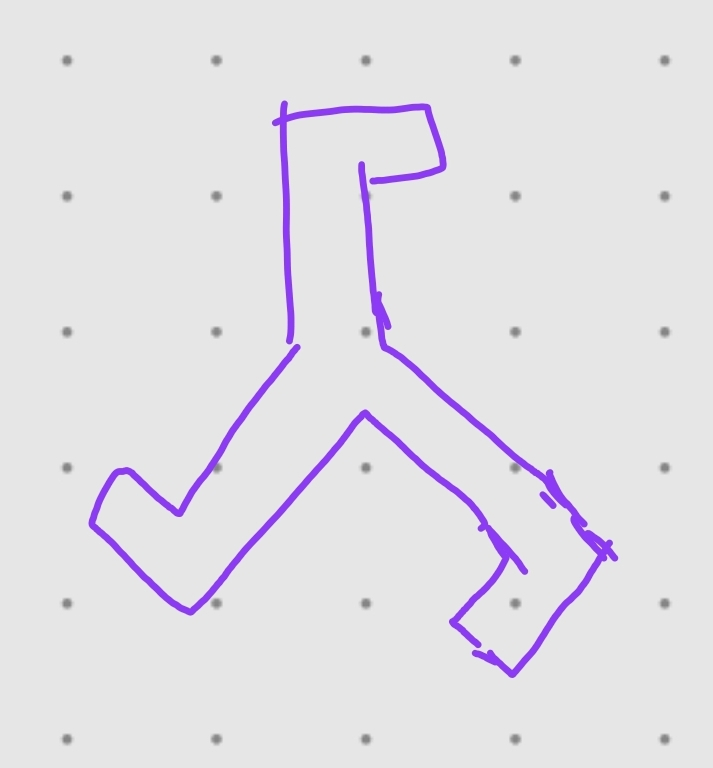
\includegraphics[width=0.3\linewidth]{5.3.1.jpg}
	\caption{The group of symmetries associated with this are identity, rotation about center by $120^\circ$, by $240^\circ$}
	\label{fig:enter-label}
\end{figure}

\begin{sol}[\textbf{Q6.4.1}]
	Let $U$ and $V$ be groups with operations $\cdot_U$ and $\cdot_V$ respectively and $a\in U$ and $a'$ be it's inverse. Let the function $\phi : U \rightarrow V$ be a homomorphism. Then
	\begin{align}
		\phi(a\cdot_U a') & = \phi(a)\cdot_V \phi(a')  \\
		\phi(e_U)         & = \phi(a) \cdot_V \phi(a') \\
		e_V               & = \phi(a) \cdot_V \phi(a') \\
	\end{align}
	since we know that $\phi(e_U)=e_V$ where $e$ is identity. Similarly we can show that
	\begin{align}
		e_V                             & = \phi(a')\cdot_V\phi(a)       \\
		\implies \phi(a)\cdot_V\phi(a') & = e_V = \phi(a')\cdot_V\phi(a) \\
		\implies \phi(a')               & = (\phi(a))'
	\end{align}
	Thus, homomorphism takes inverse of an element ($a$) to inverse of it's image.
\end{sol}

\begin{sol}[\textbf{Q6.4.2}]
	Let $a$, $b \in K$. Then $\phi(a)=\phi(b)=e_V$. Also
	\begin{align}
		\phi(a\cdot_U b) & = \phi(a)\cdot_V\phi(b) \\
		                 & = e_V                   \\
		\implies a\cdot b \in K
	\end{align}
	Thus, $K$ is a group under same operation as of $U$ thus is a subgroup of $U$.
\end{sol}

\begin{sol}[\textbf{Q6.4.3}]
	Let $a$, $b \in H$, i.e $\exists a_0$, $b_0 \in U$ such that $\phi(a_0) = a$ and $\phi(b_0) = b$.
	Then
	\begin{align}
		\phi(a_0\cdot_U b_0) & =
		\phi(a_0)\cdot_V\phi(b_0)                                                                        \\
		                     & = a\cdot_Vb                                                               \\
		\implies             & \exists c_0\in U (a_0\cdot_Ub_0) \text{ such that } \phi(c_0) = a\cdot_Vb \\
		\implies a\cdot_Vb   & \in V
	\end{align}
	Thus, $K$ forms a subgroup of $V$, known as image of $\phi$.
\end{sol}
\end{document}
